\documentclass[11pt,compress,t,notes=noshow, xcolor=table]{beamer}
\documentclass[11pt,compress,t,notes=noshow, xcolor=table]{beamer}
\usepackage[]{graphicx}\usepackage[]{color}
% maxwidth is the original width if it is less than linewidth
% otherwise use linewidth (to make sure the graphics do not exceed the margin)
\makeatletter
\def\maxwidth{ %
  \ifdim\Gin@nat@width>\linewidth
    \linewidth
  \else
    \Gin@nat@width
  \fi
}
\makeatother

\definecolor{fgcolor}{rgb}{0.345, 0.345, 0.345}
\newcommand{\hlnum}[1]{\textcolor[rgb]{0.686,0.059,0.569}{#1}}%
\newcommand{\hlstr}[1]{\textcolor[rgb]{0.192,0.494,0.8}{#1}}%
\newcommand{\hlcom}[1]{\textcolor[rgb]{0.678,0.584,0.686}{\textit{#1}}}%
\newcommand{\hlopt}[1]{\textcolor[rgb]{0,0,0}{#1}}%
\newcommand{\hlstd}[1]{\textcolor[rgb]{0.345,0.345,0.345}{#1}}%
\newcommand{\hlkwa}[1]{\textcolor[rgb]{0.161,0.373,0.58}{\textbf{#1}}}%
\newcommand{\hlkwb}[1]{\textcolor[rgb]{0.69,0.353,0.396}{#1}}%
\newcommand{\hlkwc}[1]{\textcolor[rgb]{0.333,0.667,0.333}{#1}}%
\newcommand{\hlkwd}[1]{\textcolor[rgb]{0.737,0.353,0.396}{\textbf{#1}}}%
\let\hlipl\hlkwb

\usepackage{framed}
\makeatletter
\newenvironment{kframe}{%
 \def\at@end@of@kframe{}%
 \ifinner\ifhmode%
  \def\at@end@of@kframe{\end{minipage}}%
  \begin{minipage}{\columnwidth}%
 \fi\fi%
 \def\FrameCommand##1{\hskip\@totalleftmargin \hskip-\fboxsep
 \colorbox{shadecolor}{##1}\hskip-\fboxsep
     % There is no \\@totalrightmargin, so:
     \hskip-\linewidth \hskip-\@totalleftmargin \hskip\columnwidth}%
 \MakeFramed {\advance\hsize-\width
   \@totalleftmargin\z@ \linewidth\hsize
   \@setminipage}}%
 {\par\unskip\endMakeFramed%
 \at@end@of@kframe}
\makeatother

\definecolor{shadecolor}{rgb}{.97, .97, .97}
\definecolor{messagecolor}{rgb}{0, 0, 0}
\definecolor{warningcolor}{rgb}{1, 0, 1}
\definecolor{errorcolor}{rgb}{1, 0, 0}
\newenvironment{knitrout}{}{} % an empty environment to be redefined in TeX

\usepackage{alltt}
\newcommand{\SweaveOpts}[1]{}  % do not interfere with LaTeX
\newcommand{\SweaveInput}[1]{} % because they are not real TeX commands
\newcommand{\Sexpr}[1]{}       % will only be parsed by R
\newcommand{\xmark}{\ding{55}}%


\usepackage[english]{babel}
\usepackage[utf8]{inputenc}

\usepackage{dsfont}
\usepackage{verbatim}
\usepackage{amsmath}
\usepackage{amsfonts}
\usepackage{amssymb}
\usepackage{bm}
\usepackage{csquotes}
\usepackage{multirow}
\usepackage{longtable}
\usepackage{booktabs}
\usepackage{enumerate}
\usepackage[absolute,overlay]{textpos}
\usepackage{psfrag}
\usepackage{algorithm}
\usepackage{algpseudocode}
\usepackage{eqnarray}
\usepackage{arydshln}
\usepackage{tabularx}
\usepackage{placeins}
\usepackage{tikz}
\usepackage{setspace}
\usepackage{colortbl}
\usepackage{mathtools}
\usepackage{wrapfig}
\usepackage{bm}
\usepackage{amsmath}
\usepackage{pifont}

\usetikzlibrary{shapes,arrows,automata,positioning,calc,chains,trees, shadows}
\tikzset{
  %Define standard arrow tip
  >=stealth',
  %Define style for boxes
  punkt/.style={
    rectangle,
    rounded corners,
    draw=black, very thick,
    text width=6.5em,
    minimum height=2em,
    text centered},
  % Define arrow style
  pil/.style={
    ->,
    thick,
    shorten <=2pt,
    shorten >=2pt,}
}

\usepackage{subfig}

% Defines macros and environments
\usepackage{../../style/lmu-lecture}


\let\code=\texttt
\let\proglang=\textsf

\setkeys{Gin}{width=0.9\textwidth}

\setbeamertemplate{frametitle}{\expandafter\uppercase\expandafter\insertframetitle}

% This file is included in slides and exercises

% Rarely used fontstyle for R packages, used only in 
% - forests/slides-forests-benchmark.tex
% - exercises/single-exercises/methods_l_1.Rnw
% - slides/cart/attic/slides_extra_trees.Rnw
\newcommand{\pkg}[1]{{\fontseries{b}\selectfont #1}}

% Spacing helpers, used often (mostly in exercises for \dlz)
\newcommand{\lz}{\vspace{0.5cm}} % vertical space (used often in slides)
\newcommand{\dlz}{\vspace{1cm}}  % double vertical space (used often in exercises, never in slides)
\newcommand{\oneliner}[1] % Oneliner for important statements, used e.g. in iml, algods
{\begin{block}{}\begin{center}\begin{Large}#1\end{Large}\end{center}\end{block}}

% Don't know if this is used or needed, remove?
% textcolor that works in mathmode
% https://tex.stackexchange.com/a/261480
% Used e.g. in forests/slides-forests-bagging.tex
% [...] \textcolor{blue}{\tfrac{1}{M}\sum^M_{m} [...]
% \makeatletter
% \renewcommand*{\@textcolor}[3]{%
%   \protect\leavevmode
%   \begingroup
%     \color#1{#2}#3%
%   \endgroup
% }
% \makeatother






% latex-math includes as needed
% dependencies: amsmath, amssymb, dsfont
% math spaces
\ifdefined\N
\renewcommand{\N}{\mathds{N}} % N, naturals
\else \newcommand{\N}{\mathds{N}} \fi
\newcommand{\Z}{\mathds{Z}} % Z, integers
\newcommand{\Q}{\mathds{Q}} % Q, rationals
\newcommand{\R}{\mathds{R}} % R, reals
\ifdefined\C
\renewcommand{\C}{\mathds{C}} % C, complex
\else \newcommand{\C}{\mathds{C}} \fi
\newcommand{\continuous}{\mathcal{C}} % C, space of continuous functions
\newcommand{\M}{\mathcal{M}} % machine numbers
\newcommand{\epsm}{\epsilon_m} % maximum error

% counting / finite sets
\newcommand{\setzo}{\{0, 1\}} % set 0, 1
\newcommand{\setmp}{\{-1, +1\}} % set -1, 1
\newcommand{\unitint}{[0, 1]} % unit interval

% basic math stuff
\newcommand{\xt}{\tilde x} % x tilde
\newcommand{\argmin}{\mathop{\mathrm{arg\,min}}} % argmin
\newcommand{\argmax}{\mathop{\mathrm{arg\,max}}} % argmax
\newcommand{\argminlim}{\argmin\limits} % argmin with limits
\newcommand{\argmaxlim}{\argmax\limits} % argmax with limits
\newcommand{\sign}{\operatorname{sign}} % sign, signum
\newcommand{\I}{\mathbb{I}} % I, indicator
\newcommand{\order}{\mathcal{O}} % O, order
\newcommand{\bigO}{\mathcal{O}} % Big-O Landau
\newcommand{\littleo}{{o}} % Little-o Landau
\newcommand{\pd}[2]{\frac{\partial{#1}}{\partial #2}} % partial derivative
\newcommand{\floorlr}[1]{\left\lfloor #1 \right\rfloor} % floor
\newcommand{\ceillr}[1]{\left\lceil #1 \right\rceil} % ceiling
\newcommand{\indep}{\perp \!\!\! \perp} % independence symbol

% sums and products
\newcommand{\sumin}{\sum\limits_{i=1}^n} % summation from i=1 to n
\newcommand{\sumim}{\sum\limits_{i=1}^m} % summation from i=1 to m
\newcommand{\sumjn}{\sum\limits_{j=1}^n} % summation from j=1 to p
\newcommand{\sumjp}{\sum\limits_{j=1}^p} % summation from j=1 to p
\newcommand{\sumik}{\sum\limits_{i=1}^k} % summation from i=1 to k
\newcommand{\sumkg}{\sum\limits_{k=1}^g} % summation from k=1 to g
\newcommand{\sumjg}{\sum\limits_{j=1}^g} % summation from j=1 to g
\newcommand{\summM}{\sum\limits_{m=1}^M} % summation from m=1 to M
\newcommand{\meanin}{\frac{1}{n} \sum\limits_{i=1}^n} % mean from i=1 to n
\newcommand{\meanim}{\frac{1}{m} \sum\limits_{i=1}^m} % mean from i=1 to n
\newcommand{\meankg}{\frac{1}{g} \sum\limits_{k=1}^g} % mean from k=1 to g
\newcommand{\meanmM}{\frac{1}{M} \sum\limits_{m=1}^M} % mean from m=1 to M
\newcommand{\prodin}{\prod\limits_{i=1}^n} % product from i=1 to n
\newcommand{\prodkg}{\prod\limits_{k=1}^g} % product from k=1 to g
\newcommand{\prodjp}{\prod\limits_{j=1}^p} % product from j=1 to p

% linear algebra
\newcommand{\one}{\bm{1}} % 1, unitvector
\newcommand{\zero}{\mathbf{0}} % 0-vector
\newcommand{\id}{\bm{I}} % I, identity
\newcommand{\diag}{\operatorname{diag}} % diag, diagonal
\newcommand{\trace}{\operatorname{tr}} % tr, trace
\newcommand{\spn}{\operatorname{span}} % span
\newcommand{\scp}[2]{\left\langle #1, #2 \right\rangle} % <.,.>, scalarproduct
\newcommand{\mat}[1]{\begin{pmatrix} #1 \end{pmatrix}} % short pmatrix command
\newcommand{\Amat}{\mathbf{A}} % matrix A
\newcommand{\Deltab}{\mathbf{\Delta}} % error term for vectors

% basic probability + stats
\renewcommand{\P}{\mathds{P}} % P, probability
\newcommand{\E}{\mathds{E}} % E, expectation
\newcommand{\var}{\mathsf{Var}} % Var, variance
\newcommand{\cov}{\mathsf{Cov}} % Cov, covariance
\newcommand{\corr}{\mathsf{Corr}} % Corr, correlation
\newcommand{\normal}{\mathcal{N}} % N of the normal distribution
\newcommand{\iid}{\overset{i.i.d}{\sim}} % dist with i.i.d superscript
\newcommand{\distas}[1]{\overset{#1}{\sim}} % ... is distributed as ...

% machine learning
\newcommand{\Xspace}{\mathcal{X}} % X, input space
\newcommand{\Yspace}{\mathcal{Y}} % Y, output space
\newcommand{\Zspace}{\mathcal{Z}} % Z, space of sampled datapoints
\newcommand{\nset}{\{1, \ldots, n\}} % set from 1 to n
\newcommand{\pset}{\{1, \ldots, p\}} % set from 1 to p
\newcommand{\gset}{\{1, \ldots, g\}} % set from 1 to g
\newcommand{\Pxy}{\mathbb{P}_{xy}} % P_xy
\newcommand{\Exy}{\mathbb{E}_{xy}} % E_xy: Expectation over random variables xy
\newcommand{\xv}{\mathbf{x}} % vector x (bold)
\newcommand{\xtil}{\tilde{\mathbf{x}}} % vector x-tilde (bold)
\newcommand{\yv}{\mathbf{y}} % vector y (bold)
\newcommand{\xy}{(\xv, y)} % observation (x, y)
\newcommand{\xvec}{\left(x_1, \ldots, x_p\right)^\top} % (x1, ..., xp)
\newcommand{\Xmat}{\mathbf{X}} % Design matrix
\newcommand{\allDatasets}{\mathds{D}} % The set of all datasets
\newcommand{\allDatasetsn}{\mathds{D}_n}  % The set of all datasets of size n
\newcommand{\D}{\mathcal{D}} % D, data
\newcommand{\Dn}{\D_n} % D_n, data of size n
\newcommand{\Dtrain}{\mathcal{D}_{\text{train}}} % D_train, training set
\newcommand{\Dtest}{\mathcal{D}_{\text{test}}} % D_test, test set
\newcommand{\xyi}[1][i]{\left(\xv^{(#1)}, y^{(#1)}\right)} % (x^i, y^i), i-th observation
\newcommand{\Dset}{\left( \xyi[1], \ldots, \xyi[n]\right)} % {(x1,y1)), ..., (xn,yn)}, data
\newcommand{\defAllDatasetsn}{(\Xspace \times \Yspace)^n} % Def. of the set of all datasets of size n
\newcommand{\defAllDatasets}{\bigcup_{n \in \N}(\Xspace \times \Yspace)^n} % Def. of the set of all datasets
\newcommand{\xdat}{\left\{ \xv^{(1)}, \ldots, \xv^{(n)}\right\}} % {x1, ..., xn}, input data
\newcommand{\ydat}{\left\{ \yv^{(1)}, \ldots, \yv^{(n)}\right\}} % {y1, ..., yn}, input data
\newcommand{\yvec}{\left(y^{(1)}, \hdots, y^{(n)}\right)^\top} % (y1, ..., yn), vector of outcomes
\newcommand{\greekxi}{\xi} % Greek letter xi
\renewcommand{\xi}[1][i]{\xv^{(#1)}} % x^i, i-th observed value of x
\newcommand{\yi}[1][i]{y^{(#1)}} % y^i, i-th observed value of y
\newcommand{\xivec}{\left(x^{(i)}_1, \ldots, x^{(i)}_p\right)^\top} % (x1^i, ..., xp^i), i-th observation vector
\newcommand{\xj}{\xv_j} % x_j, j-th feature
\newcommand{\xjvec}{\left(x^{(1)}_j, \ldots, x^{(n)}_j\right)^\top} % (x^1_j, ..., x^n_j), j-th feature vector
\newcommand{\phiv}{\mathbf{\phi}} % Basis transformation function phi
\newcommand{\phixi}{\mathbf{\phi}^{(i)}} % Basis transformation of xi: phi^i := phi(xi)

%%%%%% ml - models general
\newcommand{\lamv}{\bm{\lambda}} % lambda vector, hyperconfiguration vector
\newcommand{\Lam}{\bm{\Lambda}}	 % Lambda, space of all hpos
% Inducer / Inducing algorithm
\newcommand{\preimageInducer}{\left(\defAllDatasets\right)\times\Lam} % Set of all datasets times the hyperparameter space
\newcommand{\preimageInducerShort}{\allDatasets\times\Lam} % Set of all datasets times the hyperparameter space
% Inducer / Inducing algorithm
\newcommand{\ind}{\mathcal{I}} % Inducer, inducing algorithm, learning algorithm

% continuous prediction function f
\newcommand{\ftrue}{f_{\text{true}}}  % True underlying function (if a statistical model is assumed)
\newcommand{\ftruex}{\ftrue(\xv)} % True underlying function (if a statistical model is assumed)
\newcommand{\fx}{f(\xv)} % f(x), continuous prediction function
\newcommand{\fdomains}{f: \Xspace \rightarrow \R^g} % f with domain and co-domain
\newcommand{\Hspace}{\mathcal{H}} % hypothesis space where f is from
\newcommand{\fbayes}{f^{\ast}} % Bayes-optimal model
\newcommand{\fxbayes}{f^{\ast}(\xv)} % Bayes-optimal model
\newcommand{\fkx}[1][k]{f_{#1}(\xv)} % f_j(x), discriminant component function
\newcommand{\fh}{\hat{f}} % f hat, estimated prediction function
\newcommand{\fxh}{\fh(\xv)} % fhat(x)
\newcommand{\fxt}{f(\xv ~|~ \thetav)} % f(x | theta)
\newcommand{\fxi}{f\left(\xv^{(i)}\right)} % f(x^(i))
\newcommand{\fxih}{\hat{f}\left(\xv^{(i)}\right)} % f(x^(i))
\newcommand{\fxit}{f\left(\xv^{(i)} ~|~ \thetav\right)} % f(x^(i) | theta)
\newcommand{\fhD}{\fh_{\D}} % fhat_D, estimate of f based on D
\newcommand{\fhDtrain}{\fh_{\Dtrain}} % fhat_Dtrain, estimate of f based on D
\newcommand{\fhDnlam}{\fh_{\Dn, \lamv}} %model learned on Dn with hp lambda
\newcommand{\fhDlam}{\fh_{\D, \lamv}} %model learned on D with hp lambda
\newcommand{\fhDnlams}{\fh_{\Dn, \lamv^\ast}} %model learned on Dn with optimal hp lambda
\newcommand{\fhDlams}{\fh_{\D, \lamv^\ast}} %model learned on D with optimal hp lambda

% discrete prediction function h
\newcommand{\hx}{h(\xv)} % h(x), discrete prediction function
\newcommand{\hh}{\hat{h}} % h hat
\newcommand{\hxh}{\hat{h}(\xv)} % hhat(x)
\newcommand{\hxt}{h(\xv | \thetav)} % h(x | theta)
\newcommand{\hxi}{h\left(\xi\right)} % h(x^(i))
\newcommand{\hxit}{h\left(\xi ~|~ \thetav\right)} % h(x^(i) | theta)
\newcommand{\hbayes}{h^{\ast}} % Bayes-optimal classification model
\newcommand{\hxbayes}{h^{\ast}(\xv)} % Bayes-optimal classification model

% yhat
\newcommand{\yh}{\hat{y}} % yhat for prediction of target
\newcommand{\yih}{\hat{y}^{(i)}} % yhat^(i) for prediction of ith targiet
\newcommand{\resi}{\yi- \yih}

% theta
\newcommand{\thetah}{\hat{\theta}} % theta hat
\newcommand{\thetav}{\bm{\theta}} % theta vector
\newcommand{\thetavh}{\bm{\hat\theta}} % theta vector hat
\newcommand{\thetat}[1][t]{\thetav^{[#1]}} % theta^[t] in optimization
\newcommand{\thetatn}[1][t]{\thetav^{[#1 +1]}} % theta^[t+1] in optimization
\newcommand{\thetahDnlam}{\thetavh_{\Dn, \lamv}} %theta learned on Dn with hp lambda
\newcommand{\thetahDlam}{\thetavh_{\D, \lamv}} %theta learned on D with hp lambda
\newcommand{\mint}{\min_{\thetav \in \Theta}} % min problem theta
\newcommand{\argmint}{\argmin_{\thetav \in \Theta}} % argmin theta

% densities + probabilities
% pdf of x
\newcommand{\pdf}{p} % p
\newcommand{\pdfx}{p(\xv)} % p(x)
\newcommand{\pixt}{\pi(\xv~|~ \thetav)} % pi(x|theta), pdf of x given theta
\newcommand{\pixit}[1][i]{\pi\left(\xi[#1] ~|~ \thetav\right)} % pi(x^i|theta), pdf of x given theta
\newcommand{\pixii}[1][i]{\pi\left(\xi[#1]\right)} % pi(x^i), pdf of i-th x

% pdf of (x, y)
\newcommand{\pdfxy}{p(\xv,y)} % p(x, y)
\newcommand{\pdfxyt}{p(\xv, y ~|~ \thetav)} % p(x, y | theta)
\newcommand{\pdfxyit}{p\left(\xi, \yi ~|~ \thetav\right)} % p(x^(i), y^(i) | theta)

% pdf of x given y
\newcommand{\pdfxyk}[1][k]{p(\xv | y= #1)} % p(x | y = k)
\newcommand{\lpdfxyk}[1][k]{\log p(\xv | y= #1)} % log p(x | y = k)
\newcommand{\pdfxiyk}[1][k]{p\left(\xi | y= #1 \right)} % p(x^i | y = k)

% prior probabilities
\newcommand{\pik}[1][k]{\pi_{#1}} % pi_k, prior
\newcommand{\lpik}[1][k]{\log \pi_{#1}} % log pi_k, log of the prior
\newcommand{\pit}{\pi(\thetav)} % Prior probability of parameter theta

% posterior probabilities
\newcommand{\post}{\P(y = 1 ~|~ \xv)} % P(y = 1 | x), post. prob for y=1
\newcommand{\postk}[1][k]{\P(y = #1 ~|~ \xv)} % P(y = k | y), post. prob for y=k
\newcommand{\pidomains}{\pi: \Xspace \rightarrow \unitint} % pi with domain and co-domain
\newcommand{\pibayes}{\pi^{\ast}} % Bayes-optimal classification model
\newcommand{\pixbayes}{\pi^{\ast}(\xv)} % Bayes-optimal classification model
\newcommand{\pix}{\pi(\xv)} % pi(x), P(y = 1 | x)
\newcommand{\piv}{\bm{\pi}} % pi, bold, as vector
\newcommand{\pikx}[1][k]{\pi_{#1}(\xv)} % pi_k(x), P(y = k | x)
\newcommand{\pikxt}[1][k]{\pi_{#1}(\xv ~|~ \thetav)} % pi_k(x | theta), P(y = k | x, theta)
\newcommand{\pixh}{\hat \pi(\xv)} % pi(x) hat, P(y = 1 | x) hat
\newcommand{\pikxh}[1][k]{\hat \pi_{#1}(\xv)} % pi_k(x) hat, P(y = k | x) hat
\newcommand{\pixih}{\hat \pi(\xi)} % pi(x^(i)) with hat
\newcommand{\pikxih}[1][k]{\hat \pi_{#1}(\xi)} % pi_k(x^(i)) with hat
\newcommand{\pdfygxt}{p(y ~|~\xv, \thetav)} % p(y | x, theta)
\newcommand{\pdfyigxit}{p\left(\yi ~|~\xi, \thetav\right)} % p(y^i |x^i, theta)
\newcommand{\lpdfygxt}{\log \pdfygxt } % log p(y | x, theta)
\newcommand{\lpdfyigxit}{\log \pdfyigxit} % log p(y^i |x^i, theta)

% probababilistic
\newcommand{\bayesrulek}[1][k]{\frac{\P(\xv | y= #1) \P(y= #1)}{\P(\xv)}} % Bayes rule
\newcommand{\muk}{\bm{\mu_k}} % mean vector of class-k Gaussian (discr analysis)

% residual and margin
\newcommand{\eps}{\epsilon} % residual, stochastic
\newcommand{\epsv}{\bm{\epsilon}} % residual, stochastic, as vector
\newcommand{\epsi}{\epsilon^{(i)}} % epsilon^i, residual, stochastic
\newcommand{\epsh}{\hat{\epsilon}} % residual, estimated
\newcommand{\epsvh}{\hat{\epsv}} % residual, estimated, vector
\newcommand{\yf}{y \fx} % y f(x), margin
\newcommand{\yfi}{\yi \fxi} % y^i f(x^i), margin
\newcommand{\Sigmah}{\hat \Sigma} % estimated covariance matrix
\newcommand{\Sigmahj}{\hat \Sigma_j} % estimated covariance matrix for the j-th class

% ml - loss, risk, likelihood
\newcommand{\Lyf}{L\left(y, f\right)} % L(y, f), loss function
\newcommand{\Lypi}{L\left(y, \pi\right)} % L(y, pi), loss function
\newcommand{\Lxy}{L\left(y, \fx\right)} % L(y, f(x)), loss function
\newcommand{\Lxyi}{L\left(\yi, \fxi\right)} % loss of observation
\newcommand{\Lxyt}{L\left(y, \fxt\right)} % loss with f parameterized
\newcommand{\Lxyit}{L\left(\yi, \fxit\right)} % loss of observation with f parameterized
\newcommand{\Lxym}{L\left(\yi, f\left(\bm{\tilde{x}}^{(i)} ~|~ \thetav\right)\right)} % loss of observation with f parameterized
\newcommand{\Lpixy}{L\left(y, \pix\right)} % loss in classification
\newcommand{\Lpiy}{L\left(y, \pi\right)} % loss in classification
\newcommand{\Lpiv}{L\left(y, \piv\right)} % loss in classification
\newcommand{\Lpixyi}{L\left(\yi, \pixii\right)} % loss of observation in classification
\newcommand{\Lpixyt}{L\left(y, \pixt\right)} % loss with pi parameterized
\newcommand{\Lpixyit}{L\left(\yi, \pixit\right)} % loss of observation with pi parameterized
\newcommand{\Lhy}{L\left(y, h\right)} % L(y, h), loss function on discrete classes
\newcommand{\Lhxy}{L\left(y, \hx\right)} % L(y, h(x)), loss function on discrete classes
\newcommand{\Lr}{L\left(r\right)} % L(r), loss defined on residual (reg) / margin (classif)
\newcommand{\lone}{|y - \fx|} % L1 loss
\newcommand{\ltwo}{\left(y - \fx\right)^2} % L2 loss
\newcommand{\lbernoullimp}{\ln(1 + \exp(-y \cdot \fx))} % Bernoulli loss for -1, +1 encoding
\newcommand{\lbernoullizo}{- y \cdot \fx + \log(1 + \exp(\fx))} % Bernoulli loss for 0, 1 encoding
\newcommand{\lcrossent}{- y \log \left(\pix\right) - (1 - y) \log \left(1 - \pix\right)} % cross-entropy loss
\newcommand{\lbrier}{\left(\pix - y \right)^2} % Brier score
\newcommand{\risk}{\mathcal{R}} % R, risk
\newcommand{\riskbayes}{\mathcal{R}^\ast}
\newcommand{\riskf}{\risk(f)} % R(f), risk
\newcommand{\riskdef}{\E_{y|\xv}\left(\Lxy \right)} % risk def (expected loss)
\newcommand{\riskt}{\mathcal{R}(\thetav)} % R(theta), risk
\newcommand{\riske}{\mathcal{R}_{\text{emp}}} % R_emp, empirical risk w/o factor 1 / n
\newcommand{\riskeb}{\bar{\mathcal{R}}_{\text{emp}}} % R_emp, empirical risk w/ factor 1 / n
\newcommand{\riskef}{\riske(f)} % R_emp(f)
\newcommand{\risket}{\mathcal{R}_{\text{emp}}(\thetav)} % R_emp(theta)
\newcommand{\riskr}{\mathcal{R}_{\text{reg}}} % R_reg, regularized risk
\newcommand{\riskrt}{\mathcal{R}_{\text{reg}}(\thetav)} % R_reg(theta)
\newcommand{\riskrf}{\riskr(f)} % R_reg(f)
\newcommand{\riskrth}{\hat{\mathcal{R}}_{\text{reg}}(\thetav)} % hat R_reg(theta)
\newcommand{\risketh}{\hat{\mathcal{R}}_{\text{emp}}(\thetav)} % hat R_emp(theta)
\newcommand{\LL}{\mathcal{L}} % L, likelihood
\newcommand{\LLt}{\mathcal{L}(\thetav)} % L(theta), likelihood
\newcommand{\LLtx}{\mathcal{L}(\thetav | \xv)} % L(theta|x), likelihood
\newcommand{\logl}{\ell} % l, log-likelihood
\newcommand{\loglt}{\logl(\thetav)} % l(theta), log-likelihood
\newcommand{\logltx}{\logl(\thetav | \xv)} % l(theta|x), log-likelihood
\newcommand{\errtrain}{\text{err}_{\text{train}}} % training error
\newcommand{\errtest}{\text{err}_{\text{test}}} % test error
\newcommand{\errexp}{\overline{\text{err}_{\text{test}}}} % avg training error

% lm
\newcommand{\thx}{\thetav^\top \xv} % linear model
\newcommand{\olsest}{(\Xmat^\top \Xmat)^{-1} \Xmat^\top \yv} % OLS estimator in LM


% Lecture title always has to be there
\title{Algorithms and Data Structures}

\begin{document}

\titlemeta{% Chunk title (example: CART, Forests, Boosting, ...), can be empty
Encoding
}{% Lecture title
Machine numbers for $\Z$
}{% Relative path to title page image: Can be empty but must not start with slides/
}{% Learning goals, wrapped inside itemize environment
  \item Signed magnitude representation
  \item Excess encoding
  \item One's complement
  \item Two's complement
}



\begin{vbframe}{Machine numbers for $\Z$}

% Üblicherweise haben Prozessoren eigene Integer - Arithmetik.

% Auf 32-Bit Rechnern werden die ganzen Zahlen so kodiert:
% $$
%   x = \sum_{i=0}^{30} u_i 2^{i} \text{\hspace*{1cm} mit Bits } u_i\in\{0,1\}.
% $$
%
% Das 32. Bit wird für das Vorzeichen reserviert. Negative Zahlen werden üblicherweise
% im 2er-Komplement dargestellt.
% Dabei wird der Absolutbetrag in Bits konvertiert, dann alle Bits
% invertiert und eine 1 addiert (ohne overflow). Dies hat immense Vorteile, da
% z.B. Addition, Subtraktion und Multiplikation für vorzeichenbehaftete Zahlen
% prinzipiell genauso wie für Zahlen ohne Vorzeichen ausgeführt werden können.
% Der abgedeckte Zahlenbereich ist: $-2^{31}$ bis $2^{31} - 1$.
There are different options to represent positive and negative integers ($\Z$) by a computer:
\begin{itemize}
  \item Signed magnitude representation
  \item Excess encoding
  \item One's complement
  \item Two's complement
\end{itemize}

\lz 


Each representation has advantages and disadvantages regarding:
\begin{itemize}
  \item Symmetry of the representable value range
  \item Uniqueness of representation
  \item Execution of arithmetic operations
\end{itemize}
\end{vbframe}


\begin{vbframe}{Signed Magnitude Representation}


% Zur Kodierung von ganzen Zahlen repräsentiert jedes Bit die Stelle in einem dualen Stellenwertsystem.

If the 32nd bit is reserved for the sign on a 32-bit computer, 31 bits are available for encoding the absolute value of the number.

\begin{footnotesize}
\begin{center}
  \begin{tabular}{ c | ccccccccccc}
    & \multicolumn{11}{c}{Bit $u_i$} \\
    & sign & 31  & $\hdots$ & 8 & 7 & 6 & 5 & 4 & 3 & 2 & 1 \\
    \hline
    -1 & 1 & 0 & $\hdots$ & 0 & 0 & 0 & 0 & 0 & 0 & 0 & 1 \\
     0 & 1/0 & 0 & $\hdots$ & 0 & 0 & 0 & 0 & 0 & 0 & 0 & 0 \\
     1 & 0 & 0 & $\hdots$ & 0 & 0 & 0 & 0 & 0 & 0 & 0 & 1 \\
    51 & 0 & 0 & $\hdots$ & 0 & 0 & 1 & 1 & 0 & 0 & 1 & 1 \\
    \hline
      &  & $2^{30}$ & $\hdots$ & $2^7$ & $2^6$ & $2^5$ & $2^4$ & $2^3$ & $2^2$ & $2^1$ & $2^0$
  \end{tabular}
\end{center}
\end{footnotesize}

The number is then given by: $x = (-1)^{u_{32}}\sum_{i=1}^{31} u_i 2^{i-1}$.

The sign bit $u_{32} = 1$ indicates negative numbers.



\framebreak
\begin{itemize}
  \item Covered number range in 32-bit: $-2^{31}+1$ to $2^{31}-1$
  \item Very good readability
  \item Representation of zero not unique (e.g. problem with equality check: $-0 \neq 0$)
  \item Addition/subtraction is cumbersome, since the sign bit must be handled separately. You cannot simply write and add two numbers below each other (but this would be desirable!).
\end{itemize}
Example $7 - 3$ in 4-bit system:

\begin{center}
  \begin{tabular}{crl}
    &0111 &|(7)\\
    +&1011 &|(-3)\\\hline
    &(1)0010 &|(2)
  \end{tabular}
\end{center}

But $0010_2 \neq 4_{10}$. Implementation of addition is complicated.
\end{vbframe}


\begin{vbframe}{Machine numbers for $\Z$: Excess Code}
An option without a sign bit can be achieved by shifting the value ranges: 
All values are shifted by a bias (so that they are not negative).
\begin{footnotesize}
\begin{center}
  \begin{tabular}{ c | ccccccccccc}
      & \multicolumn{11}{c}{Bit $u_i$} \\
    %\cline{2-12}
      & 32 & 31  & $\hdots$ & 8 & 7 & 6 & 5 & 4 & 3 & 2 & 1 \\
    \hline
    $-2^{31}$    & 0 & 0 & $\hdots$ & 0 & 0 & 0 & 0 & 0 & 0 & 0 & 0 \\
    -1           & 0 & 1 & $\hdots$ & 1 & 1 & 1 & 1 & 1 & 1 & 1 & 1 \\
    0            & 1 & 0 & $\hdots$ & 0 & 0 & 0 & 0 & 0 & 0 & 0 & 0 \\
    1            & 1 & 0 & $\hdots$ & 0 & 0 & 0 & 0 & 0 & 0 & 0 & 1 \\
    %51           & 1 & 0 & $\hdots$ & 0 & 0 & 1 & 1 & 0 & 0 & 1 & 1 \\
    $2^{31}-1$   & 1 & 1 & $\hdots$ & 1 & 1 & 1 & 1 & 1 & 1 & 1 & 1 \\
    \hline
      & $2^{31}$ & $2^{30}$ & $\hdots$ & $2^7$ & $2^6$ & $2^5$ & $2^4$ & $2^3$ & $2^2$ & $2^1$ & $2^0$
  \end{tabular}
\end{center}
\end{footnotesize}

The coded number is calculated according to: $x = \sum_{i=1}^{32} u_i 2^{i-1} - 2^{31}$.

\begin{itemize}
  \item Covered number range in 32-bit: $-2^{31}$ to $2^{31} - 1$
  \item Uniqueness of zero
  \item No simple addition/subtraction of binary numbers
\end{itemize}

\end{vbframe}


\begin{vbframe}{One's complement}

A negative number $-z$ is represented by the bitwise complement of the corresponding positive number $z$.

\begin{footnotesize}
\begin{center}
  \begin{tabular}{ c | ccccccccccc}
    & \multicolumn{11}{c}{Bit $u_i$} \\
     & 32 & 31  & $\hdots$ & 8 & 7 & 6 & 5 & 4 & 3 & 2 & 1 \\
    \hline
    -51 & 1 & 1 & $\hdots$ & 1 & 1 & 0 & 0 & 1 & 1 & 0 & 0 \\
     -1 & 1 & 1 & $\hdots$ & 1 & 1 & 1 & 1 & 1 & 1 & 1 & 0 \\
     -0 & 1 & 1 & $\hdots$ & 1 & 1 & 1 & 1 & 1 & 1 & 1 & 1 \\
      0 & 0 & 0 & $\hdots$ & 0 & 0 & 0 & 0 & 0 & 0 & 0 & 0 \\
      1 & 0 & 0 & $\hdots$ & 0 & 0 & 0 & 0 & 0 & 0 & 0 & 1 \\
     51 & 0 & 0 & $\hdots$ & 0 & 0 & 1 & 1 & 0 & 0 & 1 & 1 \\
    \hline
       & $-(2^{31} - 1)$ & $2^{30}$ & $\hdots$ & $2^7$ & $2^6$ & $2^5$ & $2^4$ & $2^3$ & $2^2$ & $2^1$ & $2^0$
  \end{tabular}
\end{center}
\end{footnotesize}

The 32nd bit marks negative numbers again.
The coded number is given by: $x = \sum_{i=1}^{31} u_i 2^{i-1} - u_{32}(2^{31} - 1)$.

\framebreak

Let $\xt$ be the bitwise complement of $x$. We check the correctness of the formula: 

\vspace*{-.5cm}

\begin{eqnarray*}
  \xt &=& \sum_{i=1}^{31} \tilde u_i 2^{i-1} - \tilde u_{32}(2^{31} - 1) \\
  &=& \sum_{i=1}^{31} \underbrace{(1 - u_i)}_{\text{complement}} 2^{i-1} - \underbrace{(1 - u_{32})}_{\text{complement}}{(2^{31} - 1)}\\
  &=& \sum_{i=1}^{31} 2^{i-1} - (2^{31} - 1) - \sum_{i=1}^{31} u_i 2^{i-1} + u_{32}(2^{31} - 1)\\
  &=& -1 + 2^{31} - (2^{31} - 1) - (\sum_{i=1}^{31} u_i 2^{i-1} - u_{32}(2^{31} - 1)) = - x
\end{eqnarray*}


\framebreak
\begin{itemize}
\item Covered number range in 32-bit: $-2^{31}+1$ to $2^{31}-1$.
\item Very easy conversion from positive to negative and vice versa by inverting all bits.
\item The representation of zero is not unique.
\item Addition / subtraction works better here than in the signed magnitude representation. But it is still not trivial, since the sum needs to be corrected (by subsequently adding the carry bit as a 1).
\end{itemize}

Example: $7 - 3$ in 4-bit system:

\begin{center}
  \begin{tabular}{crl}
    &0111  &|(7)\\
    +&1100  &|(-3)\\\hline
    &(1)0011 &| Carry-Bit \\
    +&0001 &| add 1\\\hline
    &0100&|(4)
  \end{tabular}
\end{center}

\framebreak

Why adding a $1$?

\begin{center}
\begin{tabular}{l}
% $\,\,$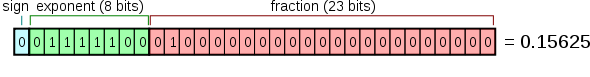
\includegraphics{32bit} \\[0.15cm]
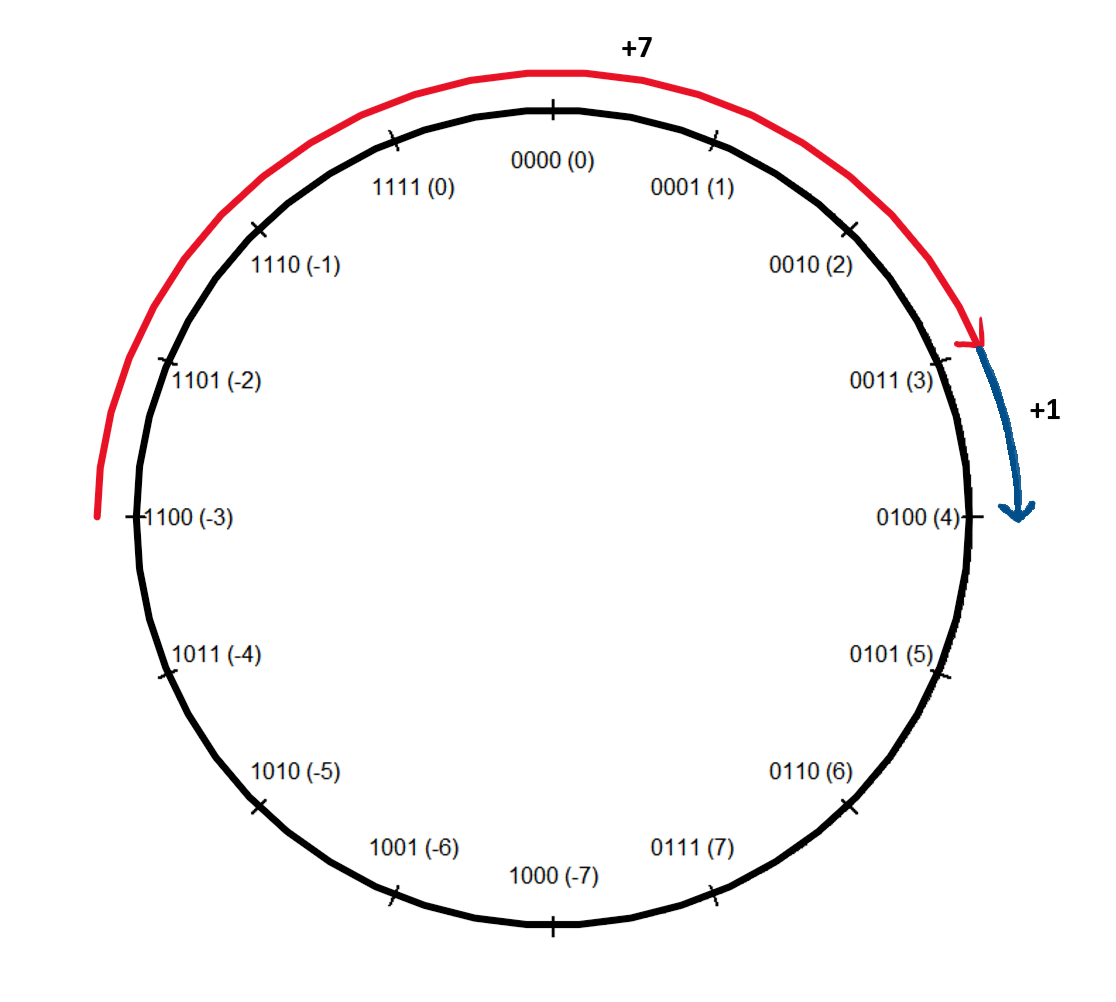
\includegraphics[width=0.4\paperwidth]{figure_man/1complement}
\end{tabular}
\end{center}

\vspace{-0.5cm}
\begin{itemize}
  \item Because of the $0$ being represented twice, a $1$ must be added when overflowing the $0$, so that the result is correct.
\end{itemize}

% <<>>=
% #1's complement
%  library(circular)
%  MyIntToBit <- function(x, dig) {
%      i <- 0L
%      string <- numeric(dig)
%      while (x > 0) {
%          string[dig - i] <- x %% 2L
%          x <- x %/% 2L
%          i <- i + 1L
%      }
%      string
%  }
%  y = lapply(0:(2^4 - 1), function(x) MyIntToBit(x,4))
%  y = lapply(y, function(x) paste(x, collapse = ""))
%  y = unlist(y)
%
%  y = paste(y, paste0("(", c(0:7, -7:-1, 0), ")"))
%
%  x = circular(seq(0, 2*pi - pi/8, pi/8))
%  plot(x, axes = FALSE, ticks = TRUE, type="n")
%  axis.circular(at=circular(seq(0, 2*pi - pi/8, pi/8), rotation = "clock", zero = 4 * pi/8),
%                labels = y, lwd = 2, tcl = 0.05)
%
% #2's complement
%  y = lapply(0:(2^4 - 1), function(x) MyIntToBit(x,4))
%  y = lapply(y, function(x) paste(x, collapse = ""))
%  y = unlist(y)
%
%  y = paste(y, paste0("(", c(0:7, -8:-1), ")"))
%
%  x = circular(seq(0, 2*pi - pi/8, pi/8))
%  plot(x, axes = FALSE, ticks = TRUE, type="n")
%  axis.circular(at=circular(seq(0, 2*pi - pi/8, pi/8), rotation = "clock", zero = 4 * pi/8),
%                labels = y, lwd = 2, tcl = 0.05)
%
% @

% \framebreak
%
% Allgemein
%
% \begin{eqnarray*}
%   \xt + x &=& \sum_{i=1}^{31} (u_i + \tilde u_i) 2^{i-1} - (u_{32} + \tilde u_{32})(2^{31} - 1)
% \end{eqnarray*}
%
% wobei
%
% $$
% (u_i + \tilde u_i) 2^{i-1}= \begin{cases}0 \cdot 2^{i-1} & \quad \text{wenn }u_i + \tilde u_i = 0 \\
% 1 \cdot 2^{i-1} & \quad \text{wenn }u_i + \tilde u_i = 1 \\
% 1 \cdot 2^{i} + 0 \cdot 2^{i-1} & \quad \text{wenn }u_i + \tilde u_i = 2 \text{ (Übertrag!)}
% \end{cases}
% $$

\end{vbframe}

\begin{vbframe}{Two's complement}

With the two's complement, negative numbers are formed by determining the one's complement and adding an additional 1.

\lz 

Example: conversion of $-51_{10}$:
\begin{footnotesize}
\begin{center}
  \begin{tabular}{ c | ccccccccccc}
      & \multicolumn{11}{c}{Bit $u_i$} \\
    %\cline{2-12}
      & 32 & 31  & $\hdots$ & 8 & 7 & 6 & 5 & 4 & 3 & 2 & 1 \\
    \hline
    $|-51_{10}|$  & 0 & 0 & $\hdots$ & 0 & 0 & 1 & 1 & 0 & 0 & 1 & 1 \\
    invert & 1 & 1 & $\hdots$ & 1 & 1 & 0 & 0 & 1 & 1 & 0 & 0 \\
    add 1 & 1 & 1 & $\hdots$ & 1 & 1 & 0 & 0 & 1 & 1 & 0 & 1 \\
    \hline
      & $-2^{31}$ & $2^{30}$ & $\hdots$ & $2^7$ & $2^6$ & $2^5$ & $2^4$ & $2^3$ & $2^2$ & $2^1$ & $2^0$
  \end{tabular}
\end{center}
\end{footnotesize}

\framebreak


Example: two's complement
\begin{footnotesize}
\begin{center}
  \begin{tabular}{ c | ccccccccccc}
      & \multicolumn{11}{c}{Bit $u_i$} \\
    %\cline{2-12}
      & 32 & 31  & $\hdots$ & 8 & 7 & 6 & 5 & 4 & 3 & 2 & 1 \\
    \hline
    $-2^{31}$    & 1 & 0 & $\hdots$ & 0 & 0 & 0 & 0 & 0 & 0 & 0 & 0 \\
    -51          & 1 & 1 & $\hdots$ & 1 & 1 & 0 & 0 & 1 & 1 & 0 & 1 \\
    -1           & 1 & 1 & $\hdots$ & 1 & 1 & 1 & 1 & 1 & 1 & 1 & 1 \\
    0            & 0 & 0 & $\hdots$ & 0 & 0 & 0 & 0 & 0 & 0 & 0 & 0 \\
    1            & 0 & 0 & $\hdots$ & 0 & 0 & 0 & 0 & 0 & 0 & 0 & 1 \\
    51           & 0 & 0 & $\hdots$ & 0 & 0 & 1 & 1 & 0 & 0 & 1 & 1 \\
    $2^{31}-1$   & 0 & 1 & $\hdots$ & 1 & 1 & 1 & 1 & 1 & 1 & 1 & 1 \\
    \hline
      & $-2^{31}$ & $2^{30}$ & $\hdots$ & $2^7$ & $2^6$ & $2^5$ & $2^4$ & $2^3$ & $2^2$ & $2^1$ & $2^0$
  \end{tabular}
\end{center}
\end{footnotesize}

The coded number is then: $x = \sum_{i=1}^{31} u_i 2^{i-1} - u_{32} 2^{31}$.

\framebreak
\begin{itemize}
\item Covered number range in 32-bit: $-2^{31}$ to $2^{31} - 1$
\item Not easy to read anymore. But big advantages for the computer.
\item Unique representation of $0$.
\item Addition / subtraction works as desired. As long as you stay in the number range, you can simply write and add two numbers below each other (the carry bit is ignored).
\end{itemize}
Example: $7 - 3$ in a 4-bit system:


\begin{center}
  \begin{tabular}{crl}
    &0111  &|(7)\\
    +&1101  &|(-3)\\\hline
    &(1)0100&|(4)
  \end{tabular}
\end{center}

\framebreak
The carry bit can simply be ignored here, since the representation of the $0$ is unique:

\vspace{-0.5cm}
\begin{center}
\begin{tabular}{l}
% $\,\,$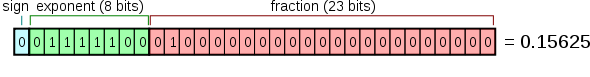
\includegraphics{32bit} \\[0.15cm]
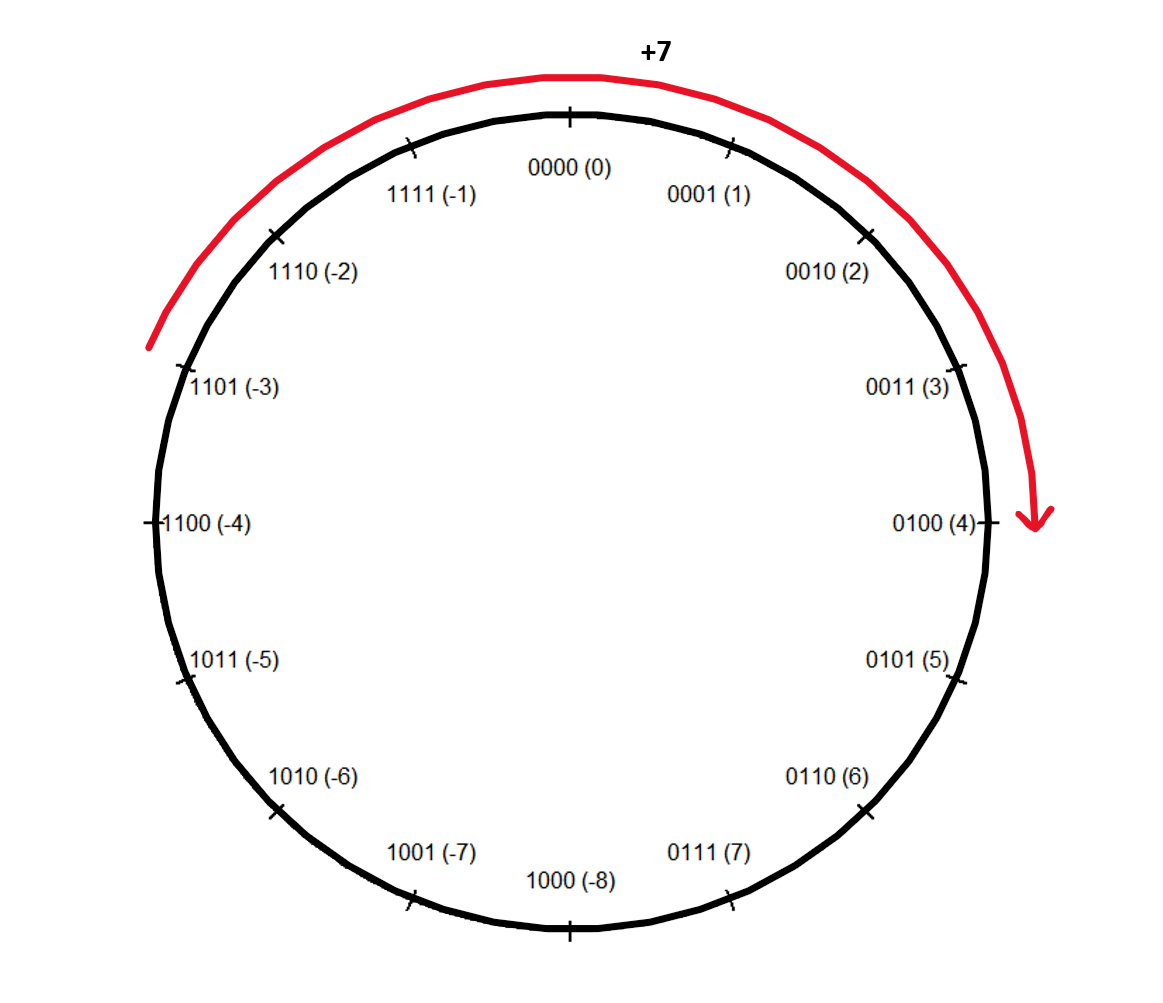
\includegraphics[width=0.4\paperwidth]{figure_man/2complement}
\end{tabular}
\end{center}

\vspace{-0.5cm}

\begin{itemize}
\item Caution when leaving the number range:
\item Example: $0011 \text{ (3)} + 0101 \text{ (5)} = 1000 \text{ (-8)}$
\end{itemize}

% \begin{center}
%   \begin{tabular}{crl}
%     &0011  &|(3)\\
%     +&0101  &|(5)\\\hline
%     &1000&|(-8)
%   \end{tabular}
% \end{center}


% \begin{itemize}
%   \item Wegen der doppelten Darstellung der 0 muss beim Überlaufen der 0 eine 1 addiert werden, damit das Ergebnis richtig ist.
% \end{itemize}

% In \pkg{R} erfolgt die Darstellung von ganzen Zahlen durch das 2er-Komplement.
%
% Positive Zahlen werden wie bisher in Bits konvertiert.
% Stehen 32 Bit zur Verfügung, wird das 32. Bit auf 0 gesetzt.
%
% Bei negativen Zahlen wird der Absolutbetrag in Bits konvertiert, dann alle Bits
% invertiert und eine 1 addiert (ohne Overflow). Dies hat immense Vorteile, da
% z.B. Addition, Subtraktion und Multiplikation für vorzeichenbehaftete Zahlen
% prinzipiell genauso wie für Zahlen ohne Vorzeichen ausgeführt werden können.
%

%

%
%

%
% Abgedeckter Zahlenbereich: $-2^{31}$ bis $2^{31} - 1$.
% <<>>=
% print(.Machine$integer.max)
% @


\end{vbframe}

\begin{vbframe}{Integer Overflow}

\textbf{Caution:} Arithmetic operations can cause an \textbf{overflow}.
This is a common programming error in languages like  \texttt{C} and can lead to undefined behavior (e.g. wrap around).

\lz

\textbf{Example}: $(2^{31} - 1) + 1$.

In a 32-bits two's complement representation $(2^{31} - 1) + 1$ would be outside of the covered number range, since $(2^{31} - 1)$ is the largest possible number that can be represented. Adding $1$ results in $-2^{31}$ due to an integer overflow.

\lz 

\centering
\begin{tabular}{c|cccc}
$(2^{31} - 1)$ & 01111111 & 11111111 & 11111111 & 11111111 \\
$+ 1$ & 00000000 & 00000000 & 00000000 & 00000001 \\
\hline
$(-2^{31})$ & 10000000 & 00000000 & 00000000 & 00000000 \\
\end{tabular}

\framebreak

Excerpt from Wikipedia "Integer Overflow":

\lz

\emph{
On 30 April 2015, the Federal Aviation Authority announced it will order Boeing 787 operators to reset its electrical system periodically, to avoid an integer overflow which could lead to loss of electrical power and ram air turbine deployment, and Boeing is going to deploy a software update in the fourth quarter.}

\lz

\emph{When Donkey Kong breaks on level 22 it is because of an integer overflow in its time/bonus. Donkey Kong takes the level number you're on, multiplies it by 10 and adds 40. When you reach level 22 the time/bonus number is 260 which is too large for its 8-bit 256 value register so it resets itself to 0 and gives the remaining 4 as the time/bonus - not long enough to complete the level.}


\end{vbframe}

\begin{vbframe}{Machine numbers for $\Z$ in \texttt{R}}

In \texttt{R}, integers are encoded in 32-bit (also in 64-bit \texttt{R}!) by the two's complement. 

\footnotesize
\vspace{0.5cm}
\begin{verbatim}
.Machine$integer.max
## [1] 2147483647
\end{verbatim}

\vspace{0.2cm}
\begin{verbatim}
2^31 - 1
## [1] 2147483647
\end{verbatim}


\framebreak 

\footnotesize
\vspace{0.5cm}
\begin{verbatim}
intToBits(-51L)
## [1] 01 00 01 01 00 00 01 01 01 01 01 01 01 01 01 01 01 01
## [19] 01 01 01 01 01 01 01 01 01 01 01 01 01 01
\end{verbatim}

\vspace{0.2cm}
\begin{verbatim}
intToBits(51L)
## [1] 01 01 00 00 01 01 00 00 00 00 00 00 00 00 00 00 00 00
## [19] 00 00 00 00 00 00 00 00 00 00 00 00 00 00
\end{verbatim}

\vspace{0.2cm}
\begin{verbatim}
# Caution: In R the operation x^y always results in the type 'numeric'!
intToBits(2L^31L - 1L)
## [1] 01 01 01 01 01 01 01 01 01 01 01 01 01 01 01 01 01 01
## [19] 01 01 01 01 01 01 01 01 01 01 01 01 01 00
\end{verbatim}



\framebreak 
\normalsize
In \texttt{R}, integer overflows are caught and set to NA.
\lz
\footnotesize
\begin{verbatim}
.Machine$integer.max + 1 
## [1] 2147483648
\end{verbatim}

\vspace{0.2cm}
\begin{verbatim}
str(.Machine$integer.max + 1) 
## num 2.15e+09
\end{verbatim}

\vspace{0.2cm}
\begin{verbatim}
str(.Machine$integer.max + 1L)
## Warning in .Machine$integer.max + 1L: NAs produced by 
   integer overflow
## int NA
\end{verbatim}


\end{vbframe}
\normalsize

\begin{vbframe}
\frametitle{R in 64-bit systems}
\begin{itemize}
  \item In 2010, the 64-bit version of \texttt{R} was released.
  \item \textbf{But:} integers are still encoded in 32-bit.
  \item The largest integer in \texttt{R} is thus about 2 billion.
  \item When indexing vectors longer than about 2 billion, \texttt{R} uses a trick:
  \begin{itemize}
    \item By using floating point numbers in double precision, integers can be represented reliably within the value range $(-2^{53}, 2^{53})$.
    \item Beyond that, not all integers are covered!
    \item In \texttt{R} you can index with floating point numbers:
  \end{itemize}
\end{itemize}

\footnotesize
\lz
\begin{verbatim}
c(1,2,3)[1.7]
## [1] 1
\end{verbatim}

\end{vbframe}

\endlecture
\end{document}

% https://github.com/SurajGupta/r-source/blob/56becd21c75d104bfec829f9c23baa2e144869a2/src/library/stats/src/cov.c

